\documentclass[conference]{IEEEtran}
% Include all packages from file.
% Article template for Imperial College Software Engineering for Industry course
% Based on report template for Mälardalen University
% Original template can be found:
% https://www.overleaf.com/latex/templates/ieee-bare-demo-template-for-conferences/ypypvwjmvtdf
% Template file structure organised by: Emil Persson
% The following packages should follow the IEEE conference guidelines.

\usepackage[utf8]{inputenc}
\usepackage[T1]{fontenc}

% Graphics
\usepackage{graphicx, float, subfigure, blindtext}
\newcommand\IEEEhyperrefsetup{
    bookmarks=true,bookmarksnumbered=true,%
    colorlinks=true,linkcolor={red},citecolor={red},urlcolor={black}%
}

% Preferred hyperref setup, Michael Shell
\usepackage[\IEEEhyperrefsetup, pdftex]{hyperref}
\usepackage[backend=bibtex,style=ieee,natbib=true]{biblatex} % Use the bibtex backend with the authoryear citation style (which resembles APA)
\addbibresource{refs.bib}
% These packages must be at the end
\usepackage[nolist,nohyperlinks]{acronym}
\usepackage{cleveref}
% Remove section first paragraph indent
\usepackage{titlesec}
\titlespacing*{\section}{0pt}{*1}{*1}
\titlespacing*{\subsection}{0pt}{*1}{*1}
\renewcommand{\thesubsubsection}{\arabic{subsubsection}}
\titleformat{\subsubsection}[runin]{\itshape}{\thesubsubsection)}{1em}{}[:]
\titlespacing*{\subsubsection}{\parindent}{0pt}{*1}

\usepackage[nodayofweek]{datetime}


% The article title.
\title{Detailed Case Study of \emph{Blockchain.com}, a Fast-growing Cryptocurrency Company}

% Document begins here
\begin{document}

    \author{Nicolás D'Cotta -- \today}

% Create the title.
    \maketitle

% Example sections, name them
% according to specific needs.
    \begin{abstract}
        Blockchain is a crypto finance house that scaled fivefold in
        employees in less than a couple of years, and is growing still.
        This article looks into the challenges it faces scaling up human and technical resources (mostly drawing from personal experience) and reflects on what works well (and what does not!) as well as how the solutions to these challenges interact with one another.

        Topics covered include microservices, combining agile with a regulated environment, the organisation's topology, Conway's Law, SRE, and incident response.
    \end{abstract}


    \section{Blockchain's Size and Business Model}\label{sec:business}

    I have worked at Blockchain for little under 2 years and during that time I was able to observe
    how the company went from about \textbf{110 employees to more than 500} at the time of writing (with many
    of the new joiners being engineers), transformed into a \textbf{remote-first organisation}~(largely because
    of the coronavirus), grew an \textbf{institutional business}, and \textbf{tripled its existing retail business}.

    The company started in 2011 as a free simple blockchain explorer~\cite{bcAbout} that later
    begun offering non-custodial online Bitcoin wallets.
    When I joined, it had around 40 million active wallets in several cryptocurrencies,
    a brokerage service (to buy and sell crypto to users), as well as a recent currency
    exchange (where users trade with each other, not unlike Coinbase~\cite{coinbasePro}).

    This is implemented with a coarse-grained microservices architecture, with some services
    being much larger than others.


    \section{Scaling Up Systems}
    We call the larger services \emph{core services}, and they are further split into modules.

    This results in a hybrid of microservices with a couple large services.
    When adding a new feature, depending on its scope and the data it needs, it is either built into
    a microservice or simply inside an existing core service.
    If, further down the line, it is decided it needs to grow further, it can get moved out of a
    core service into a new microservice.

    \subsection{Dealing With Large Services}

    Something the team noticed about the core services around 2019 is that when they were large
    enough, compilation and testing times were no longer negligible: from a commit in a feature
    branch being pushed, it took 50 minutes for the retail core service to compile and test~\footnote{
        Causes for the slow compilation time include code generation and annotation processing that were involved in the process.
    }
    (after which the branch could be merged into \texttt{master}).
    After the merge, CI took another 50 minutes to test and build again (the new merge commit
    may not be building the exact same artifact as the previous test run) to produce
    the docker image that could then be deployed.

    Developers also need to get two approving reviews in order to merge, so overall we would expect at least two hours from the moment we pushed a commit to the moment we were able to deploy it.
    These delays greatly hindered our ability to perform incident response, test-driven development (local testing took just as long), and quick iterating in general.

    It was in order to mitigate this that modules were introduced in the core services, making them as small as possible.
    The modules are dynamically linked and so compilation artifacts can now be cached for each module in CI persistent storage, which is hosted by a cloud provider and scaled dynamically with the number of concurrent builds.
    Therefore, when modifying a module, developers only need to wait for that module's compilation, its tests, and the integration tests -- binaries and test results from other modules are reused.
    Additionally, developers' build tools are given remote read access to the build cache, so their local compilation times also massively improved.

    After the modularisation of the core services and the implementation of the build cache, builds improved dramatically (most commonly down to 10 minutes per build) both locally and on CI, and core services became much easier to break up -- although, interestingly, that was not the main motivation behind the refactor.
    This shows Blockchain leveraging modularisation and cloud to scale tooling that speeds up iteration -- and therefore shortens the feedback loop with customers for a feature (in line with Lean practices) and facilitates practices such as TDD\@.

    \subsection{Zero-downtime}

    Unlike more traditional markets and trading platforms, crypto markets are usually always open.
    Therefore, downtime translates to losses for the business, so zero-downtime deployability is
    very desirable.

    While there is no company-wide policy, the platform team tries to always have 2 instances
    of every service running at all times.
    This allows for the following:

    \begin{itemize}
        \newcommand{\entry}[1]{\item[] \hspace{-1em}\textbf{#1}}
        \entry{Blue/Green delpoyments}~\cite{nomadBlueGreen} where one instance of the
        service at a time is updated to the new version.
        Once an instance has been serving traffic for a short while, it is marked as `healthy', and
        the next instance is updated.
        This means that even during a new release, there is always an instance serving traffic.
        \entry{Higher Availability} -- if an instance crashes, the load balancer can direct traffic
        to the other (hopefully still healthy) instance while the unhealthy one is restarted.
        \entry{Stateless Services} -- developers are aware that whatever new service they are
        writing, it will most likely be running two instances from the start.
        This encourages (but does not force) engineers to write stateless services, so they will not
        have to bother with mechanisms like leader election\footnote{
            \textbf{Leader Election} is a protocol where a cluster of servers agree on a
            `leader' among them, commonly to run tasks that cannot be parallelized~\cite{attiya2004distributed}.}.
    \end{itemize}\

    In practice, always running more than a single instance of a service from the start is a mostly
    successful policy, but there are some downsides.

    Firstly, it is costly -- plenty of microservices could cope with load on a single instance just
    fine, but still run two.
    This is mitigated with containers, as opposed to using a machine for each
    instance.

    Secondly, some services cannot easily be made stateless (examples include polling services
    and the ledger), so we must choose between a single instance or several instances with leader
    election mechanisms.
    For the sake of less downtime, the latter is usually preferred;
    which means engineers need to reason about leadership when developing these services.

    Finally, Blue/Green deployments do have a price: deployments are much slower because not
    all instances are updated at once.
    For services that take a long time to start up (5 minutes) and have lots of instances (say 15)
    it can take more than 40 minutes for the old containers to be completely phased out.
    This makes fixing urgent issues in production via deployments much slower than if old containers were stopped
    straight away.

    \subsection{Growing in a Financial Regulated Environment}\label{subsec:regulated}

    As a company operating in the finance industry, which is heavily regulated, and dealing
    with large monetary amounts;
    consistency, reliability, and accountability are at the top of Blockchain's priorities.

    For reasons explained in~\ref{subsec:ul}, we write actor-oriented code.
    This makes reasoning about capturing events easy (an event is simply a message!) and allows
    implementing Event Sourcing (ES)~\cite{fowlerES} on critical monetary services (like the ledger).

    Event Sourcing allows resiliency and consistency without having to resort to transactionality
    or retries: messages are persisted and replayed on service restarts or crashes.
    It also enables a very transparent audit trail of everything happening inside services -- one
    can just look at the persisted events.

    While in theory ES provides many benefits, in practice it proved very costly to implement.
    Very critical old code had to be re-written in an actor-oriented fashion, persisting messages adds runtime overhead, replaying them makes service startups much slower (an issue exacerbated by Blue/Green deployments), and serialisation has to be implemented for events.
    Serialisation in particular involves a lot of boilerplate code for each message class.
    To add to the complexity, modifying a state machine often involves changing the messages actors
    pass around.
    This means that then we must deal with different serialisation versions and worry about
    backwards compatibility between them.
    While the problems listed are very painful to deal with, they are a price the team willingly pays for the guarantees ES brings.


    \section{Scaling Up People}

    \subsection{Microservices to Restructure Teams}

    Moving a module inside a core service out to its own microservice can happen as the team that
    owns the macroservice grows and needs to be partitioned.
    This is the case when a feature becomes large enough to deserve its own engineer owners.

    This happened with a `crypto brokerage' service which got split off from the retail core
    service.
    Aside from partitioning the retail team in order to from a new brokerage team, the other goal of
    this migration was to achieve more fine-grained deployability: brokerage was getting releases
    more often than the core, and we wanted to be able to roll back one without rolling back the
    other -- this allowed the two teams to not step on each other's toes.
    This shows Blockchain trying to leverage Conway's Law~\cite{conwayLaw}.

    \subsection{Ubiquitous Language}\label{subsec:ul}

    Another paradigm that facilitated Blockchain's fast growth was the idea of having a
    \emph{Ubiquitous Language} (or \emph{UL})~\cite{evansDomainDrivenDesignUL, fowlerUL}.
    The goal is to have some form of documentation that describes the functioning of a `flow' (like
    the process for withdrawing crypto from the exchange).
    This from of communication should be understood by engineers as well as the product team.

    The UL we use to represent Flows are Finite State Machine (FSM) diagrams, designed to have well-named states and state transitions depending on each interaction with the user, other microservices, and external services.
    Forcing some backend teams to think of flows as Finite State Machines allows implementing
    them as actors which go through state transitions.
    Events that trigger these transitions are just messages passed around between actors.

    \phantomsection
    \label{para:busFactor}
    The ultimate purpose of introducing UL was to be able to transmit and persist knowledge
    effectively, because Blockchain had what we called a strong `bus
    factor'~\cite{bowlerTruckFactor} -- meaning that if a few, knowledgeable team members got hit by
    a bus, then the company would be in serious trouble.
    The reason for this was probably a mix of high rotation of employees due to varying competitive
    salaries in the crypto industry (so team members that remained gained seniority very quickly) and
    complex critical legacy code that only some understood.

    While the idea of UL is nothing new (\cite{evansDomainDrivenDesignUL} is from 2004) I personally
    think Blockchain took an innovative approach in that they took it to the extreme by using FSMs
    and diagrams and exposing product to them, rather than simply conforming to \emph{`a common [...]
        language between developers and users'} (as described by Martin Fowler in~\cite{fowlerUL}).

    The idea of Ubiquitous Language was successful, to some extent.
    Finite State Machine diagrams do make it very easy to communicate a flow or a feature while
    accounting for every single edge case and interaction.
    But having to design a state machine can be tedious for simple cases, and
    for complex ones it can be too time-consuming (some FSMs have `sub-FSMs' when they are too large
    to put in a single document!).
    Additionally, most developers are very used to classical object-oriented programming, and at first it is time-consuming to train them
    to write in an actor model -- it is also harder to find new hires that know the
    paradigm well.
    Furthermore, having to represent state transitions for every single side effect and call (and the
    states resulting from their failures) requires large amounts of boilerplate -- code that
    traditionally would have been a simple \emph{try-catch} in Kotlin or Java.

%    \subsection{\textsc{COVID-19} and Remote Work} TODO what would I say

    \subsection{Squads and Organisation Topology}\label{subsec:squads}

    Around June 2020, Blockchain decided to adopt Squads to organise their teams.
    The variation of squads they adopted includes a Product Owner (PO) and a Tech Lead (TL), as well as cross-functional representatives of other teams (such as Platform, Mobile, Marketing, etc).
    This organisation is similar to the one Spotify presents in~\cite{spotifySquads}, with some key differences (depicted in Fig.~\ref{fig:squad}):
    \begin{itemize}
        \item The presence of the Tech Lead.
        They are responsible for making important technical decisions (typically the ones involving compromises in cost or tech debt), coordinating engineers of different domains within a squad, and deciding which engineers are needed for this squad (this involves negotiating resources and priorities with TLs of other squads).
        \item No chapters.
        \item Guild leads are Line Managers of people in that guild.
        For example, the brokerage team has a lead that manages around 4 engineers, distributed across squads.
        \item People can exist outside of squads, in specialised service teams.
        The ledger team is a good example of this: most of the daily work does not involve a PO but rather making sure it can scale up with company growth.
        When a whole new feature does involve the ledger, a ledger team member gets pulled into that feature's squad for a period of time.
        \item A person can belong in more than a single squad.
    \end{itemize}

    \begin{figure}[h]
        \centering
        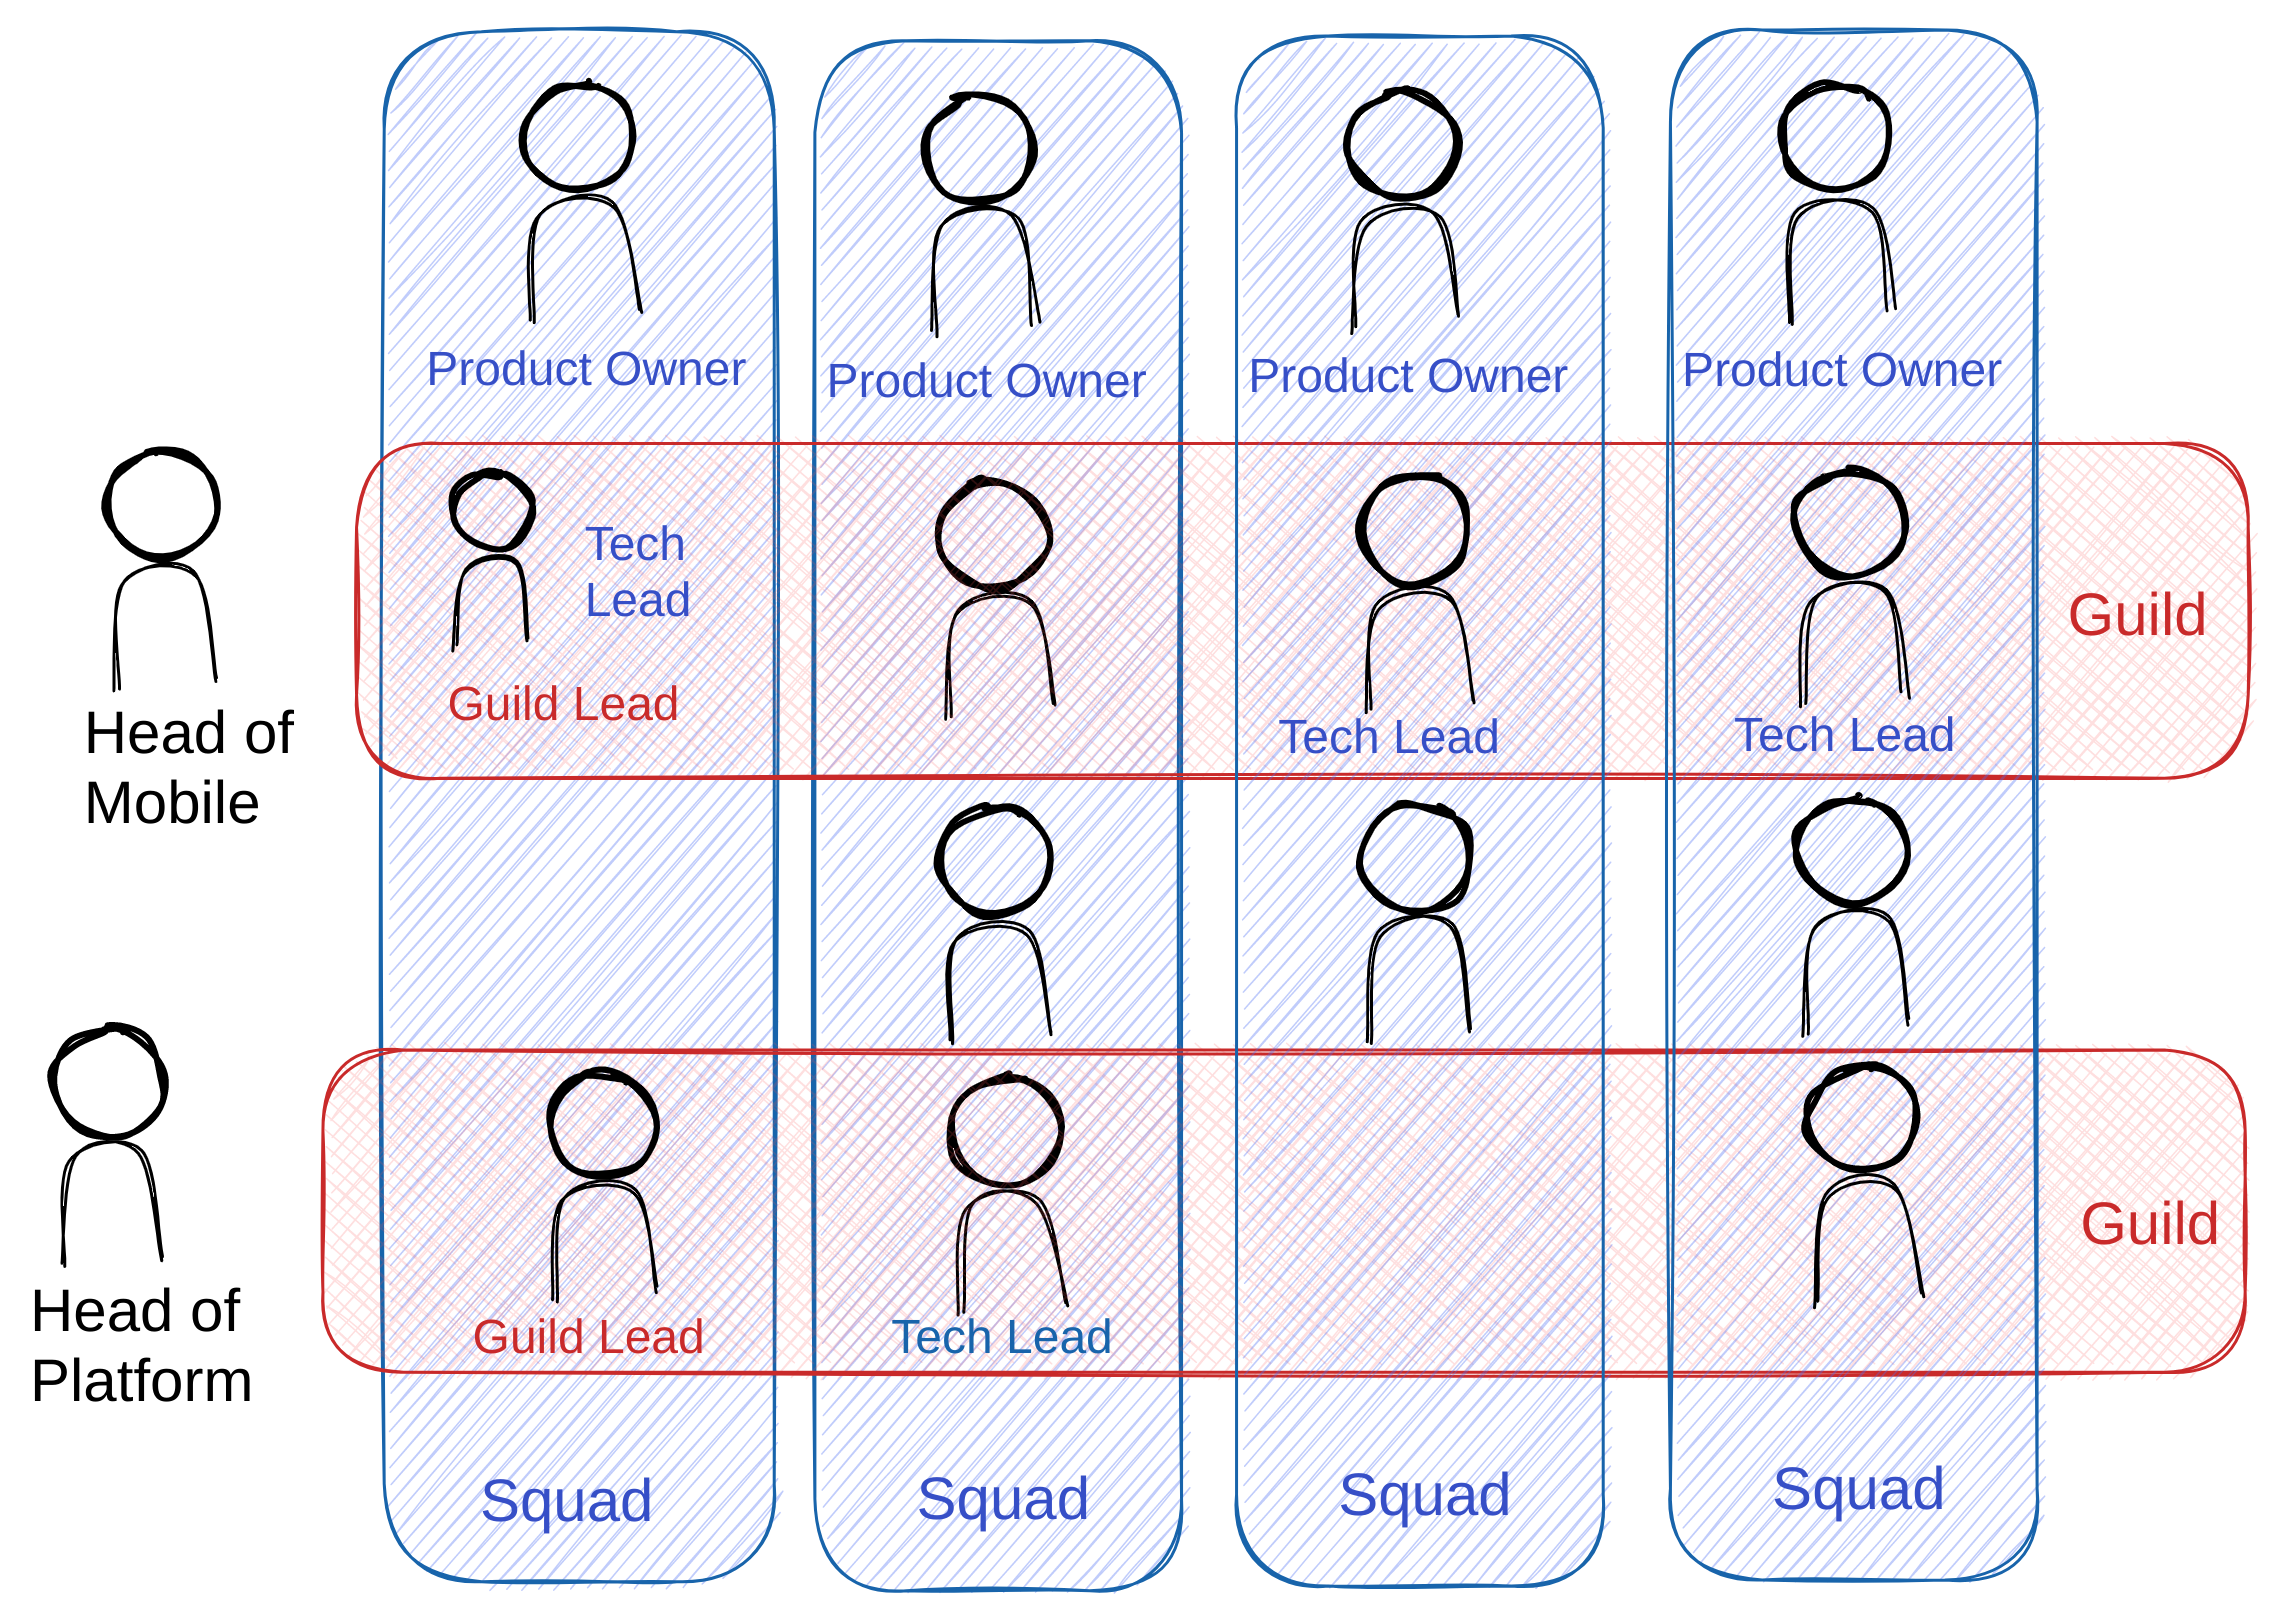
\includegraphics[width=0.94\columnwidth]{bcSquads}
        \caption{Squad Structure at Blockchain}
        \label{fig:squad}
    \end{figure}

    Motivations for this significant re-shuffling were that traditional teams had become too large to coordinate internally and that communication had become much trickier in the face of remote work.
    For example, before the migrating to squads the retail backend team (a subset of the much larger platform team) had 10 members involved in daily stand-ups.
    Such meetings only became bothersome to the team after it grew bigger than its 4 original members.
    After squads, this daily stand-up became a much more informal weekly guild meeting.

    Squads also make it easier to reason about the resources allocated for a specific goal, because they are teams built around such goals.
    As such, to allocate and distribute resources as the company's priorities change, people often get shuffled around between squads depending on where manpower is needed.
    Adopting squads worked well and this shows in that Blockchain is now a remote-first company which does not intend to go back to relying on having most of its staff in its offices.
    The main office in London shut down, and has been replaced by a much smaller one mainly composed of meeting rooms instead of desks, which staff are free to use should they wish to meet face-to-face.

    Difficulties associated with this transformation include difficulties organising large amounts of resources for projects.
    When the need for a new squad arises (because a new feature must be built, for example) staff can get allocated to it without getting deallocated from other squads.
    This results in an engineer reporting to two POs as well as a LM and sometimes struggling to reconcile their respective priorities.

    \subsection{Operations Responsibilities and SRE}

    All development teams are responsible for performing releases of their services and performing the plumbing necessary to achieve a deployment pipeline.
    The Site Reliability Engineering team (SRE) is a specialised team of developers that aims to facilitate this.
    The practice was originally pioneered by Google~\cite{googleSreIntro} and Blockchain follows it at a smaller scale.

    At Blockchain, SRE builds automated tooling that allows developers to deploy and maintain their services, but devs maintain the responsibilities of production incident response, pipeline development, releases, provisioning, etc.
    In general, SRE works \emph{as-a-service}, while also assisting for specialised setups.

    The structure of SRE within the company is portrayed in Fig.~\ref{fig:sre}.
    I personally found this organisation very productive for the following reasons:
    \begin{itemize}
        \item Developers maintain some important operations responsibilities and own the CI pipeline (critical in the release process).
        \item Developers do not need to worry about maintaining a significant part of the stack that is hidden away from them: SRE takes care of things like DNS, load balancing between instances of the same service, negotiating resources with cloud providers and maintenance of on-premises infrastructure.
        \item Developers still have freedom to achieve their desired setups without compromising with friction, and this is reflected in the diversity of practices across teams.
        Some teams perform Continuous Delivery (where the code in the \texttt{master} branch corresponds to the microservice in production), others perform releases manually via the CLI; some run JVM services, others Rust or C++;
        some services run with cloud providers while the most sensitive ones run on-premises, etc.
        \item Most tooling provided by SRE, including server provisioning, is automated, meaning communication overhead is minimal.
        % TODO revise
        In practice, having an SRE team feels a like having infrastructure as a service within the company.
        \item Teams can still achieve more complex setups with SRE as enablers
        if they desire.
        A good example is the markets team, which exceptionally pins threads to individual CPUs and performs networking bypassing the kernel in order to achieve minimal latencies.
        \item SRE have plenty of technical background to understand the cost needs of developers and negotiate compromises accordingly.
    \end{itemize}

    \begin{figure}[h]
        \centering
        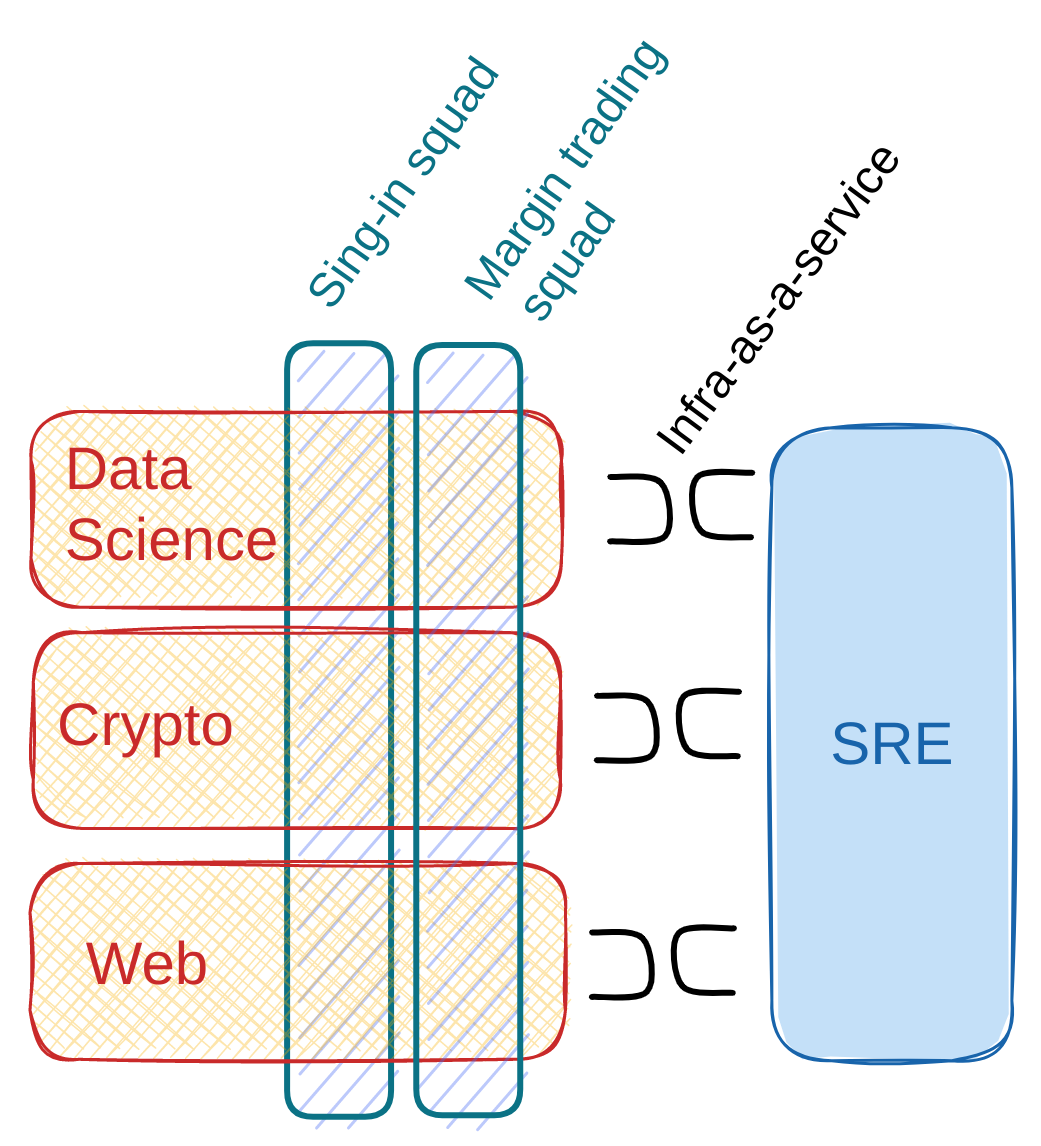
\includegraphics[width=0.67\columnwidth]{sreAsAService}
        \caption{SRE interactions with other teams\footnotemark}
        \label{fig:sre}
    \end{figure}
    \footnotetext{Not meant to properly represent a topology under Kelton's model~\cite{skelton2019topologies}.}

    Having a separate SRE team that manages lots of operational aspects of the company does include some downsides.
    The entire stack is not managed by developers which means they lack in-depth understanding of the technologies involved, which can make debugging harder.
    In particular, when a bug arises, it can be hard to determine if the root cause is at the application level (the side managed by devs: Kafka, serialisation, business logic, etc.) or at the networking level (managed by SRE).
    When this situation arises, at least one engineer from both teams is required to safely be able to rule out one or the other.


    \section{Incident Response}\label{sec:incident-response}

    Production incident response is one of the areas where Blockchain struggles to achieve results the team is fully satisfied with.

    Application monitoring is something the company started relatively doing early on and does work well: when writing new code reviewers always encourage adding metrics, which are persisted during runtime in real-time.
    The data can then be read and aggregated by an internal web client every engineer has access to (in our case, \textit{Grafana}~\cite{grafana}).
    Additionally, we perform Application Performance Monitoring (APM) thanks to a tool (specifically, \textit{Datadog}~\cite{datadogApm}) that hooks up to runtimes and performs additional real-time tracing and profiling of code segments as well as individual network requests.
    This practice of `If it moves, we track it', first developed by Etsy~\cite{etsyStatsd}, allows a great deal of observability into the platform's stability, throughput, availability, and most importantly, how it is performing with respect to its Service Level Objectives (SLOs).
    Alerting is then set up for these metrics, and the on-call engineer is paged when SLOs are not met.
    Notice the use of \emph{aggregate-driven} monitoring instead of \emph{event-driven} monitoring.

    By default, every platform engineer is on call and in the same rota (meaning they take turns in 12-hour shifts) -- this is the case because engineers change between squads and services often and maintaining rotas that reflect this has proven difficult.
    When an alert comes through, the responder triages if necessary: they escalate to a different team, page someone else, or defer until office hours in their timezone.

    While the alerting is therefore very relevant, and the observability crucial when debugging during an incident, incident response is not satisfactory for the following couple of reasons.
    Firstly, engineers get paged about services they are unfamiliar with.
    This happens because the on-call rota concerns a lot of services, so response often involves escalation to a different engineer with more knowledge in the area.
    It is another strong symptom of Blockchain's `bus factor' (see~\ref{para:busFactor}).
    Secondly, engineers get paged often.
    This is a result of having plenty of analytics and alerting in place, resulting in spurious issues triggering possibly irrelevant alerts.
    Consequently, alerts get revised often and `known' ones can even get ignored.

    No obvious solutions exist for these issues, which partly have arisen from the fact the incident response process has remained largely unchanged as the platform team grew.
    Partitioning the on-call rota is costly because it must then be maintained as developers jump from one microservice to another (which often happens informally).
    Creating a separate team specialised in incident response is a possibility that has been considered and then discarded: responders would have even less knowledge on the systems they have to fix because they would be less likely to be the same people that routinely maintain them (further suffering from the strong `bus factor').


    \section{In Retrospective}\label{sec:conclusion}

    While Blockchain is an organisation with plenty of both technical and structural issues, it has adapted relatively well to the extremely rapid growth it has seen.
    This growth has happened in the complicated environment of the extremely volatile cryptocurrency markets it operates in and with additional constraints such as tight regulation, remote work, costly downtime, and challenging technical problems in general.

    \printbibliography
\end{document}

